\section{Architektur \& Design}
\label{sec:architecture_design}

\paragraph{Primary textual contributors.}
\mbox{}\\\emph{Thomas Kretschmann}

In diesem Kapitel wird die Architektur und das dazugehörige Design von SWTcamper präsentiert. Zuerst zeigen wir, für welches Architekturmodell wir uns entschieden haben und begründen unsere Entscheidung. Dann werden wir die darauf aufbauende Umsetzung erläutern, und wie daraus individuelle Designentscheidungen abgeleitet werden können. Insbesondere werden wir auf das Design des Datenbankschemas und die Darstellung der einzelnen Entitäten eingehen. Abschließend werden die verwendeten Entwurfsmuster und Entwurfsprinzipien vorgestellt und dargestellt
erklärt.


\subsection{Architektur erklärt}
Bei der Architektur von SWTcamper haben wir uns für das Model-View-Controller Architekturmuster entschieden, da dies das Frontend vom Backend abkapselt und es ermöglicht bei gleich bleibendem Backend die grafische Nutzeroberfläche zu verändern. Das ist vor allem in dem Hinblick interesant, dass vorgesehen wird, dass zukünftige SWL-Studierende die Anwendung mit einem Web-Frontend versehen sollen.

Im Gegensatz dazu läuft die von uns gebaute Anwendung komplett lokal, wobei man sich aber vorstellen könnte die Datenbank, bzw. den Dockercontainer, der jene beinhaltet, auch auf einer örtlich entfernen Maschine anzubieten.

Durch die klare Aufteilung der zum MVC-Pattern (gut erkennbar in \ref{fig:architecture}) gehörenden Schichten war es außerdem sehr gut möglich, zugehörige Tasks klar getrennt auf Teammitglieder zu verteilen.

\begin{figure}[h]
	\centering
	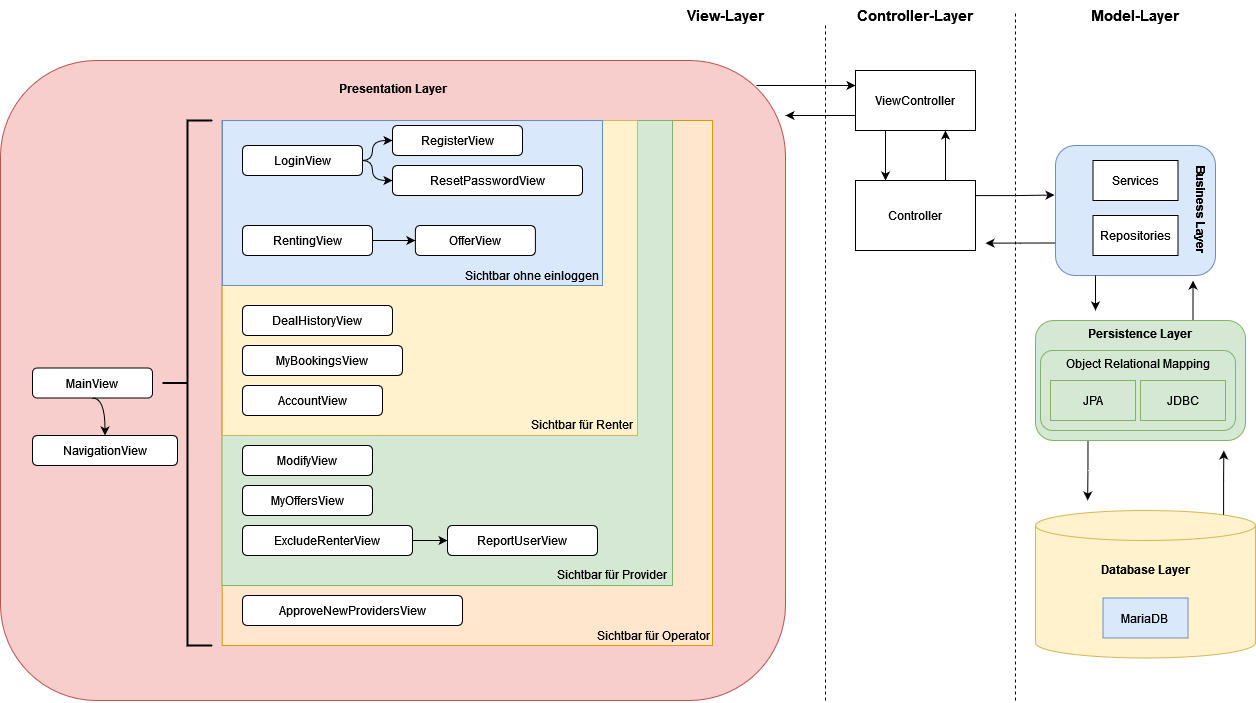
\includegraphics[width=12cm]{resources/images/architecture.drawio.png}
	\caption{Architektur}
	\label{fig:architecture}
\end{figure}

\subsubsection{Layered MVC generell}
Das Model View Controller-Pattern ist ein Architektur-, bzw. Entwurfsmuster, das einen flexiblen Programmentwurf bietet, eine spätere Änderung oder Erweiterung erleichtert und eine Wiederverwendbarkeit der einzelnen Komponenten ermöglicht.
Anwendungen, welche nach den Prinzipien von MVC gestaltet werden, bestehen aus drei austauschbaren Komponenten: 

\begin{itemize}
	\item Das Model besteht aus mehreren Model-Klassen. Jede repräsentiert eine grundlegende Einheit innerhalb der verwendeten Datenstruktur. Sie stellen darüber hinaus grundlegende Datenoperationen zur Verfügung, welche nicht unbedingt der prinzipiellen Programmlogik zugehörig sind. Dazu gehören zum Beispiel die einzelnen Entitäten auf deren Grundlage die Anwendung läuft, oder auch die Services die notwendige Werte aus der Datenbank bereitstellen und bereits zum notwendigen Grad verarbeiten können.
	
	\item View-Klassen stellen die grafische Benutzeroberfläche bereit. Die Model-Klassen stellen die angezeigten Daten zur Verfügung, eine direkte Verbindung zwischen den beiden Programmteilen existiert allerdings nicht. Der Controller informiert die Bestandteile der Oberflächendarstellung über Änderungen am Model und diese passen die angezeigten Inhalte bei Bedarf an.
	
	\item Die Controller-Klassen fungieren als Verbindungsstück zwischen View- und Model-Bestandteilen. Aktionen der Nutzer leitet die View zum Controller weiter, welcher die dahinterstehende Programmlogik ausführt. Die Logik informiert einzelne Views im Bedarfsfall über Änderungen am Model, um eine passende Reaktion auf diese zu ermöglichen.
\end{itemize}

\subsubsection{JavaFX (view)}
JavaFX ist ein Open-Source-Framework, das zum Erstellen von grafischen Benutzeroberflächen (GUI) verwendet wird. Wir haben in SWTcamper die Funktion von JavaFX verwendet, die es ermöglicht, den Ansichtsteil vollständig in FXML-Dateien zu definieren. 
Lediglich in für die dynamischen Programmteile wurden die Views programmatsch erzeugt (z.B. für die Liste an verfügbaren Anzeigen oder das Operator-Dashboard). Die View wird dann während der Laufzeit des Programms unter Verwendung der FXML-Dateien und JavaFX erstellt. Die ViewController sind die Controller der einzelnen Views, die sich nicht nur um das Event-Handling kümmern, sondern auch von den \"richtigen\" Controllern Daten anfordern und weiterleiten.

\subsubsection{Spring boot (view, controller, model)}
Spring Boot ist ein Open-Source-Framework, das viele Funktionalitäten zur Entwicklung einer eigenständigen Anwendung bietet. Es vereinfacht den Softwareentwicklungsprozess, indem es die Komplexität reduziert und eine klare Struktur bietet. Es kommt dabei in unserem Fall in jeder Schicht des MVC-Patterns zum Einsatz.

Damit das Framework weiß, wie es mit jeder Klasse umgeht, gibt es Annotationen die es Spring Boot ermöglichen, die erforderliche Umgebung für die Klassen zu erstellen. Ein Beispiel dafür ist die Annotation @Service, die über jeder unserer Serviceklassen platziert wird, oder @Component, das über jedem Controller zum Einsatz kommt.

Einfach nur Spring Boot zu benutzen garantiert keine Qualität, aber es bietet eine Struktur, die es einfacher macht, qualitative Software zu entwickeln Fehler zu vermeiden.

\subsubsection{JPA (model)}
In Kombination mit Spring Boot ermöglicht uns die Java Persistence API die Konvertierung von Java-Objekten in
Datenbankobjekte und umgekehrt. Durch Annotationen in den Entitätsklassen lassen sich diverse Einstellungen vornehmen, um das gewünschte Datenbankschema automatisch zu implementieren.

\subsubsection{Docker (model)}
Docker ist eine Open-Source-Software, die es uns ermöglicht, Anwendungen in einem virtuellen Container-Umgebung auszuführen. Viele Softwareanbieter bieten bereits vorkonfigurierte Images an, es ermöglichen, dass ihre Anwendung in einer containerisierten Docker-Umgebung ausgeführt wird. 
Wir haben Docker verwendet, um unsere Datenbank MariaDB darin auszuführen.

\subsubsection{MariaDB (model)}
MariaDB ist eine relationale Open-Source-Datenbank. Wir verwenden es, um unsere Daten konsistent zu speichern. MariaDB bietet auch ein eigenes Docker-Image an, was es zu einer guten Wahl für unsere Anwendung macht.

\subsection{Von der Architektur zum Design}
Um zu verstehen welche Komponenten wir für die Anwendung brauchen und wie wir am besten vorgehen haben wir im Rahmen des ersten Sprints ein Use Case Diagramm (\ref{fig:use-case-diagram}) und ein ein ER-Diagramm (\ref{fig:er-diagram}) angefertigt, welche sich im Laufe des Projekts verändert haben.

\begin{figure}[h]
	\centering
	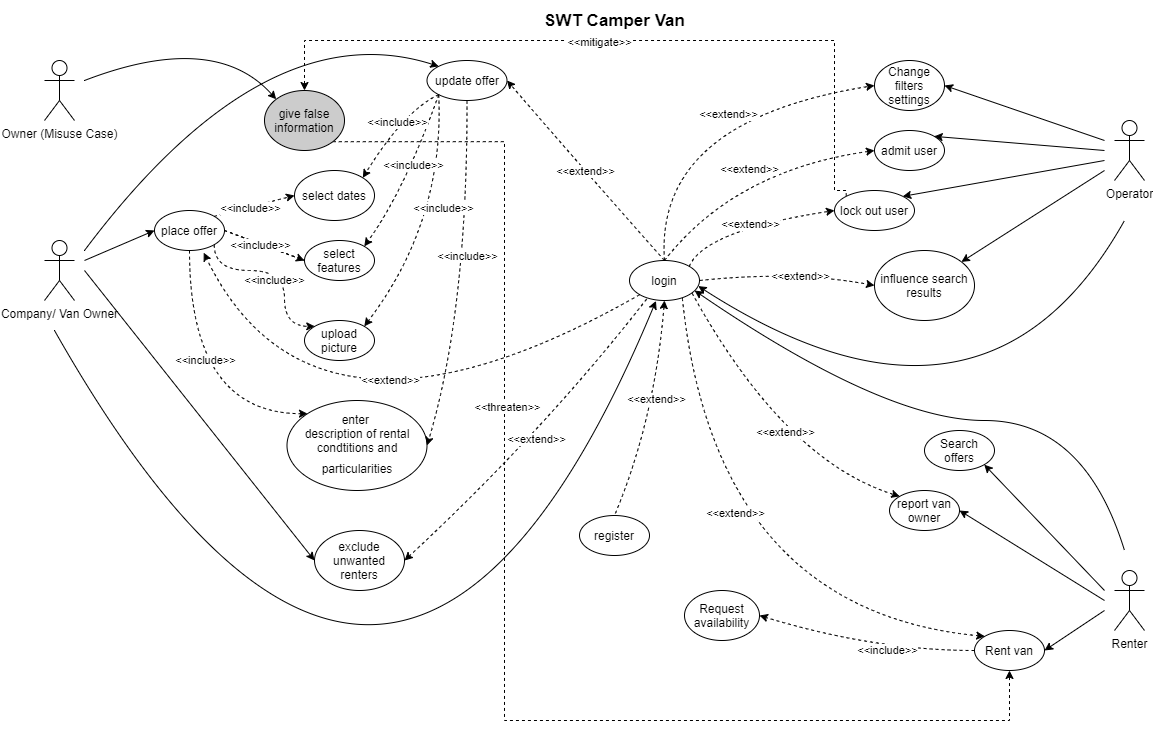
\includegraphics[width=15cm]{resources/images/use-case-diagram.png}
	\caption{Use Case Diagramm}
	\label{fig:use-case-diagram}
\end{figure}

\paragraph{Grundstruktur}
Das Herzstück von SWTcamper ist die MainView und ihr zugehöriger ViewController, die bei Programmstart direkt von App.java (Startpunkt für JavaFX Anwendungen) aufgerufen wird. Sie beinhaltet über Imports alle anderen FXML-Views, die über den Controller abhängig vom NavigationViewController hinzugefügt oder entfernt werden. (in \ref{fig:architecture} versucht dar zu stellen) Bei Programmstart wird über die Methode changeView() zuerst die RentingView geladen, die alle verfügbaren Anzeigen beinhaltet. Dazu wird das sich in der MainView befindende AnchorPane \"mainStage\" zuerst komplett geleert und anschließend mit der genannten RentingView gefüllt. Drückt der Nutzer nun einen Button in der NavigationView (Buttons werden abhängig von der UserRole angezeigt (ebenfalls aus \ref{fig:architecture} zu entnehmen)), wird über deren ViewController der MainViewController beauftragt das gleiche Vorgehen für die neu ausgewählte View zu wiederholen. Um die Views voneinander zu unterscheiden, muss in die genannte Methode changeView() ein passender String übergeben werden (z.B. \"home\" für die RentingView oder \"history\" für die DealHistoryView). Da zu Programmstart bereits alle ViewController initialziert werden, müssen in den MainViewController auch alle anderen ViewController importiert werden, damit man für jeden einzeln eine Reload-Methode aufrufen kann.

\subsection{Klassendiagramm}
% TODO
\begin{figure}[h]
	\centering
	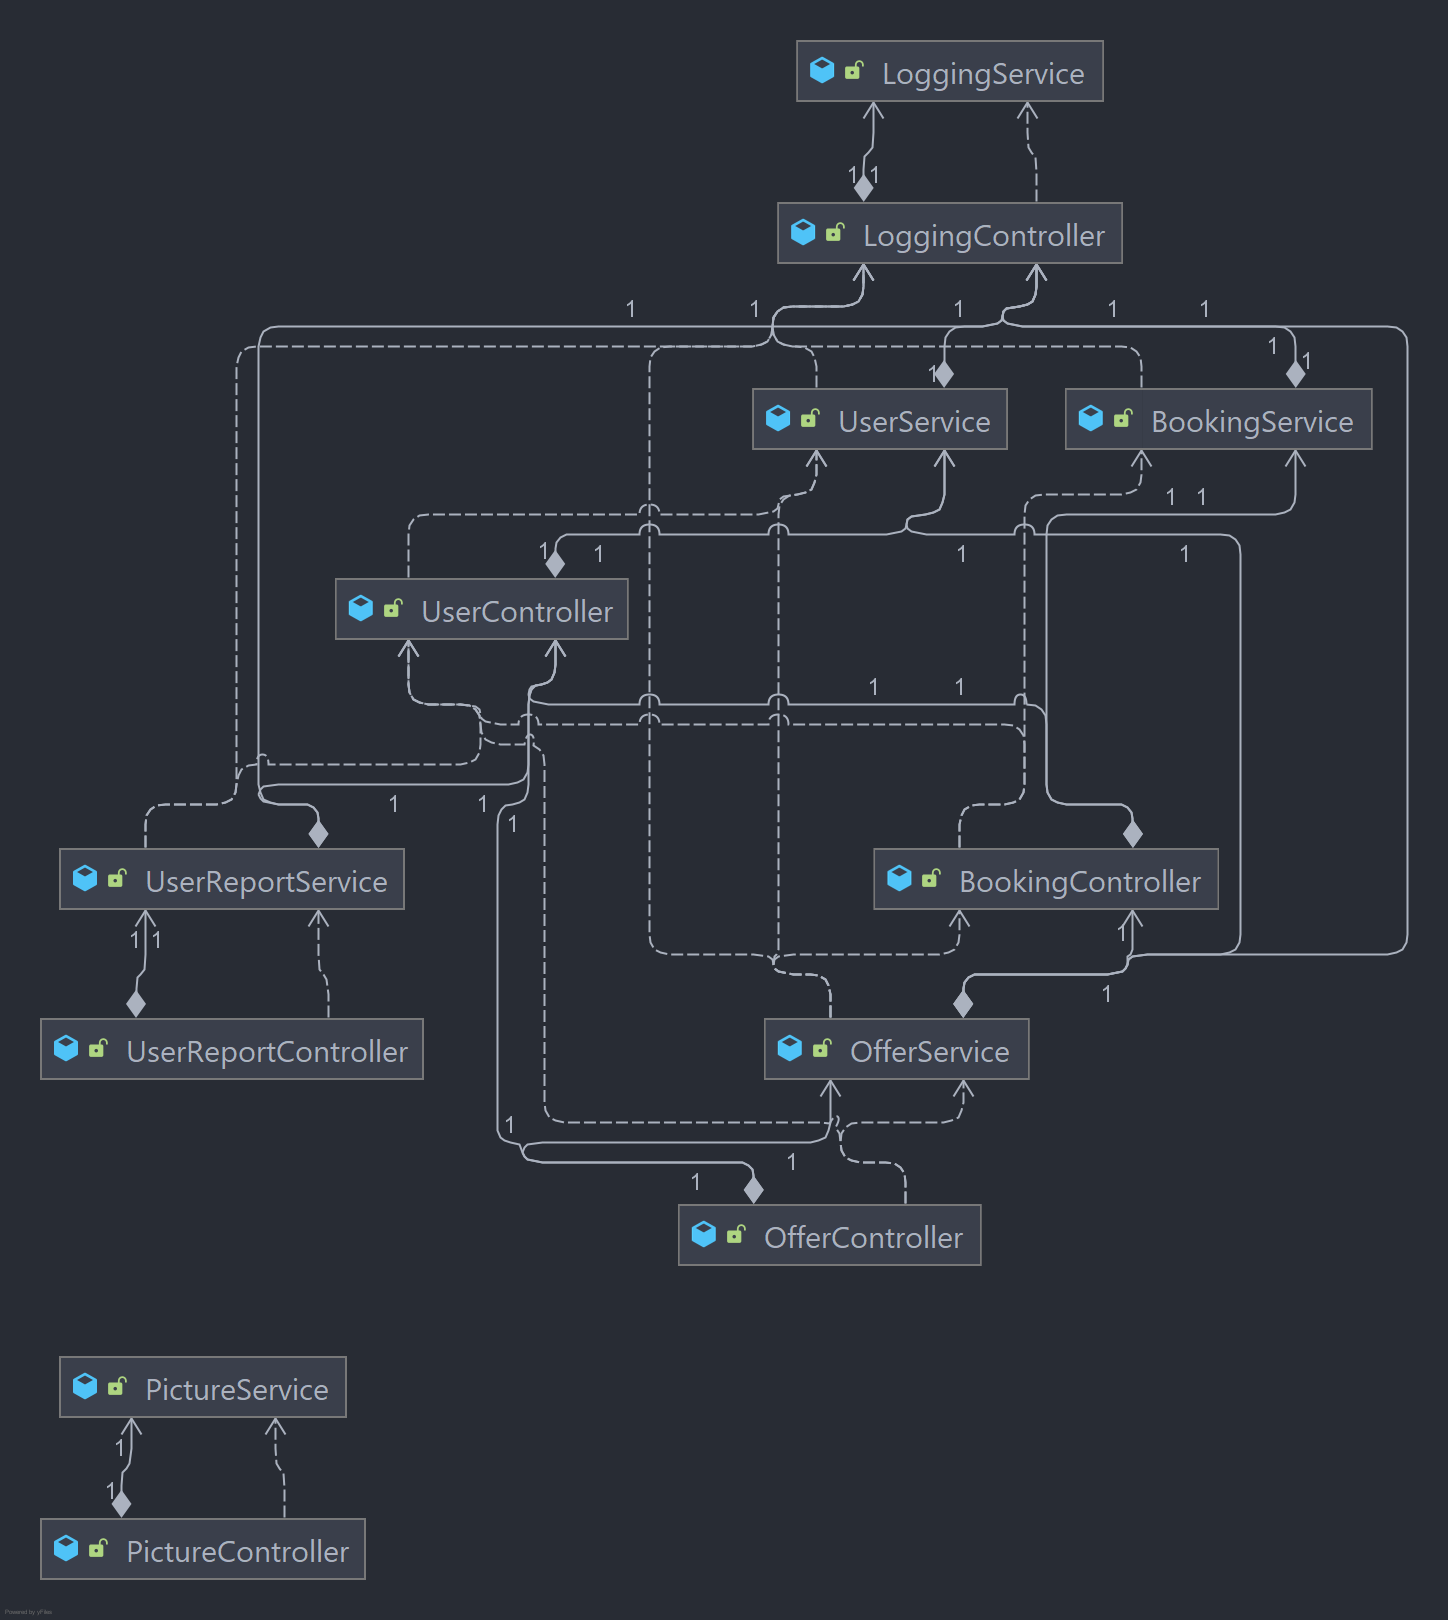
\includegraphics[width=8cm]{resources/images/class diagrams/class-diagram_controller-services.png}
	\caption{Klassendiagramm Controller-Services}
	\label{fig:cd:controller-services}
\end{figure}
\begin{figure}[h]
	\centering
	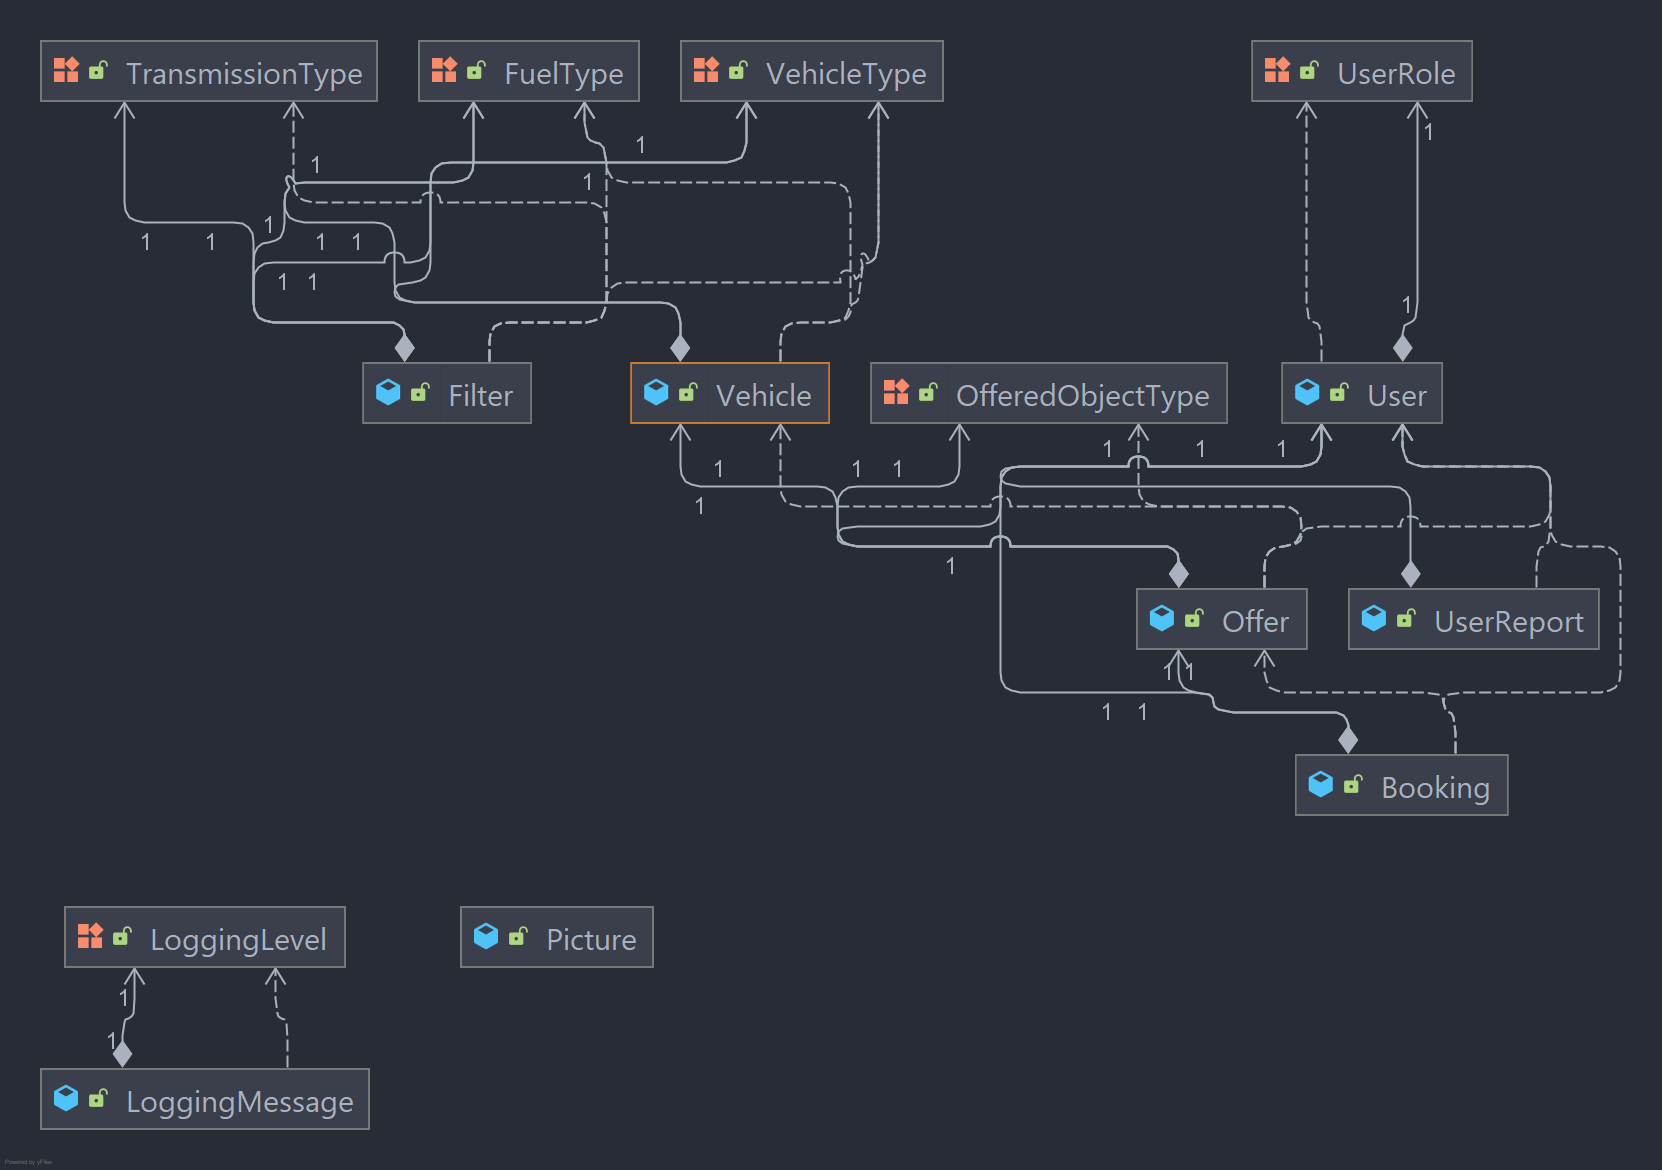
\includegraphics[width=8cm]{resources/images/class diagrams/class-diagram_entities.png}
	\caption{Klassendiagramm Entities}
	\label{ffig:cd:entities}
\end{figure}

\subsection{Datenmodell \& Designentscheidungen}
% TODO
\begin{figure}[h]
	\centering
	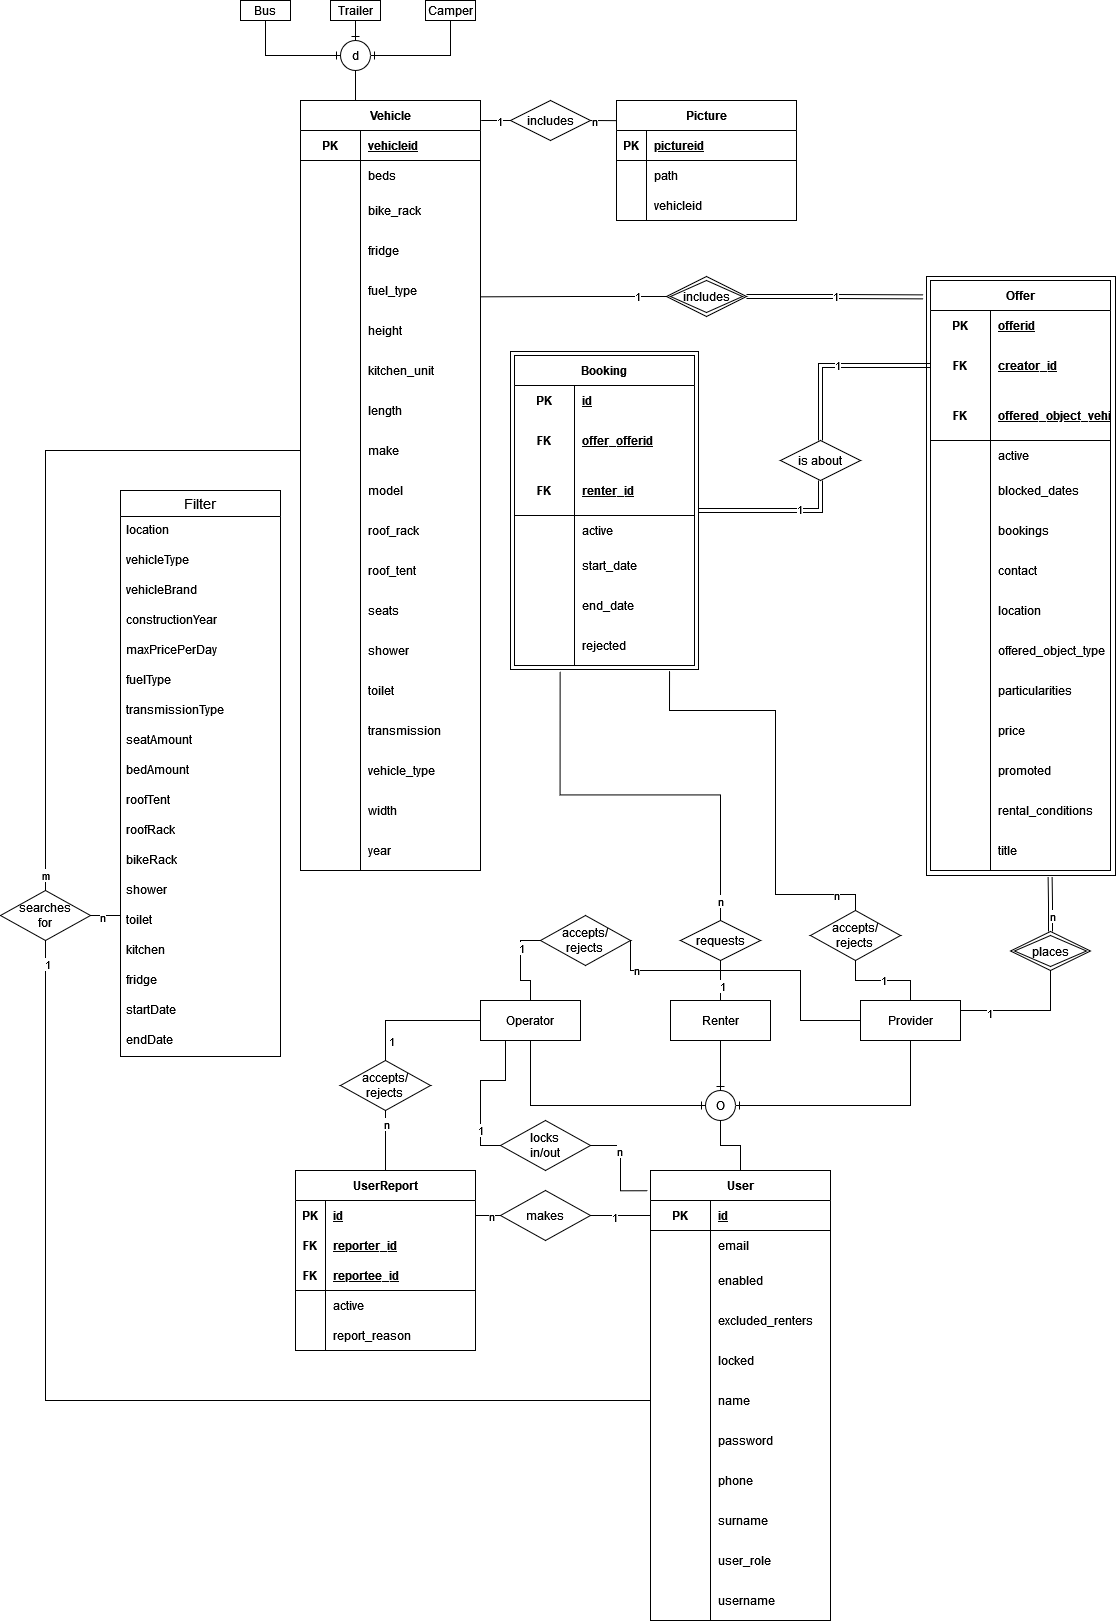
\includegraphics[width=15cm]{resources/images/ER-diagram.drawio.png}
	\caption{Entity Relationship Diagram}
	\label{fig:er-diagram}
\end{figure}

\paragraph{Booking}
Die Booking-Klasse wird benötigt um einen User an eine Anzeige zu binden. Dazu besitzt sie eine ID die (durch die Annotationen @Id und @GeneratedValue) automatisch von der Datenbank generiert wird, einen User der die zugehörige Anzeige mieten möchte, die genannte Anzeige selbst, ein Startdatum und ein Enddatum. Des weiteren gibt es die beiden boolschen Felder active und rejected. Eine Buchung wird mit active = false erzeugt und bleibt solange inaktiv bis sie angenommen wird; sollte sie abgelehnt werden, wird das ebenfalls mit false erzeugte Feld rejected auf true gesetzt. Die Kombination dieser beiden Werte wird an mehreren Stellen der Anwendung gebraucht um Zustände festzustellen:

\begin{tabular}{|c|c|c|c|}
	\hline
	&  & \multicolumn{2}{c|}{active} \\
	\hline
	&  & true & false \\
	\hline
	rejected & true & \begin{tabular}[c]{@{}c@{}}Anzeige wurde frühzeitig beendet,\\wird im Angebotsverlauf gelistet\end{tabular} & / \\
	\hline
	& false & \begin{tabular}[c]{@{}c@{}}Anzeige kann nicht bearbeitet \\oder gelöscht werden\end{tabular} & \begin{tabular}[c]{@{}c@{}}Anzeige erscheint bei Provider in \\``Neue Anfrage zu Angebot'' \\(noch nicht im Verlauf)\end{tabular} \\
	\hline
\end{tabular}

\paragraph{Filter}
Die Filter-Klasse ist die einzige Entitätsklasse in SWTcamper, die nicht in der Datenbank gespeichert wird. In ihr kommen alle Felder aus Offer und Vehicle vor, die für eine gute Suche benötigt werden. Bei Start der Suche wird eine neue Filterinstanz erzeugt und die notwendigen Felder gesetzt. Diese Instanz wird dann dem OfferController übergeben, der damit die Liste aller Anzeigen filtert und eine neue Liste mit zur Filterinstanz passenden Anzeigen zurückgibt.

\paragraph{LoggingMessage}
LoggingMessages werden von fast allen Services aus generiert und werden benötigt um Geschehnisse nachverfolgen zu können. Eine Liste an LoggingMessages kann als Operator über die AccountView eingesehen und als log-Datei heruntergeladen werden. Da alle vorkommenden LoggingMessages auch in der Datenbank gespeichert werden besitzt jede eine eindeutige und automatisch generierte ID und einen Zeitstempel zu dem sie ertellt wurde. Der Enum LoggingLevel gibt an wie wichtig die LoggingMessage ist (INFO, WARNING, ERROR) und es gibt außerdem noch eine Nachricht damit der Einseher weiß um was es geht.

\paragraph{Offer}
Die Offerklasse wurde mit der Vehicleklasse zusammen als erstes in SWTcamper implementiert. Im Laufe der Entwicklung wurde sie allerdings erweitert und verbessert. Sie wird benötigt um Anzeigen abzubilden - einer der Grundlagen von SWTcamper. Objekte dieser Klasse besitzen eine von der Datenbank automatisch generierte ID, einen User der der Ersteller der Anzeige ist, Titel, Abholort, Kontaktdaten über die der Ersteller erreichbar sein möchte, Besonderheiten über die Anzeige (wie zum Beispiel Dinge die nicht über SWTcamper bereits abgedeckt werden) und einen Preis. Über active kann der Ersteler angeben, ob die Anzeige öffentlich gelistet werden soll und wenn prmoted true ist, wird die Anzeige in der Liste hervorgehoben; diese Funktion kann nur von Operatoren verändert werden, ist aber für alle Nutzer sichtbar. Des weiteren enthält jede Anzeige natürlich auch ein fest dazugehöriges Vehicle-Objekt mit all seinen Werten und jeweils Listen für blockierte Daten zu denen die Anzeige nicht gebucht werden kann, nicht überschneidenden Buchungen und rentalConditions, mit denen der Ersteller Bedingungen festlegt, an die sich der Mieter zu halten hat. \\
Das Feld offeredObjectType wird in unserer Version von SWTcamper nicht weiter genutzt; es wäre allerdings möglich die Anwendung hier zu erweitern.

\paragraph{Picture}
Urspünglich war geplant, dass die in SWTcamper für die Vehicles gespeicherten Bilder komplett in die Datenbank geladen werden; dabei gab es allerdings viele Probleme den richtigen Datentyp zu finden und es kam zu vielen Fehlern, dass die Datenbank keine Objekte dieser Größe speichern könne. Deswegen sind wir als nächstes darauf umgestiegen, im Vehicle Objekt eine Liste an Pfaden zu speichern. Diese Liste war allerdings ab ungefähr drei Bildern ebenfalls zu lang für die Datenbank. \\
Als Lösung haben wir deswegen ein eigenes Repository für die Bilder erstellt. Dabei enthält jeder Eintrag neben der obligatorischen ID den Pfad zu dem Bild und die ID zu dem Vehicle zu dem es zuzuordnen ist. \\
Durch diesen Ansatz können Bilder leider nur lokal gespeichert werden und funktierien nicht in einem verteilten System. Da unsere Anwendung allerdings sowieso nur die Anforderung hatte, lokal zu laufen, war das für diesen Rahmen in Ordnung.

\paragraph{User}
Die Userklasse besitzt neben einer automatisch erzeugten ID außerdem Attribute für den Nutzernamen, Vor- und Nachnamen, Emailadresse, Telefonnummer und Passwort. Das Attribut userRole gibt an welche Rolle der Nutzer bei Nutzung der Anwendung einnimmt, und welche Befugnisse er dadurch hat (vgl. View-Abbildung in \ref{fig:architecture}). Damit zusammenhängend gibt es außerdem das Attribut enabled, das nur auf false gesetzt wird wenn sich ein Nutzer als Provider neu registriert, da es eine Aforderung war, dass diese Personen zuerst geprüft werden sollen bevor sie neue Anzeigen erstellen können. Solange ein Nutzer die Rolle des Providers hat und enabled auf false steht, hat er die gleichen Befugnisse und Möglichkeiten wie die Nutzerrolle Renter. \\


% TODO
Long id
String username
String name
String surname
String email
String phone
String password
UserRole userRole
boolean locked
boolean enabled
ArrayList<Long> excludedRenters

\paragraph{UserReport}
UserReports werden benötigt, damit ein Nutzer (ab UserRole Provider) einen anderen melden kann. Ein abgesendeter UserReport wird dann in der Datenbank gespeichert (hat wieder eine automatisch generierte ID) und hat dabei ein boolean Feld active, das auf true gesetzt ist, bis der Report von einem Operator bearbeitet (angenommen oder abgewiesen) wird. Um dem entscheidenden Operator seine Entscheidung einfacher zu machen, beinhaltet jeder UserReport sowohl den Nutzernamen des Meldenden, als auch des Gemeldeten und eine Nachricht, warum der Meldende die Meldung eingereicht hat.

\paragraph{Vehicle}
% TODO
long vehicleID
VehicleType vehicleType
String make
String model
String year
double length
double width
double height
FuelType fuelType
String transmission
int seats
int beds
boolean roofTent
boolean roofRack
boolean bikeRack
boolean shower
boolean toilet
boolean kitchenUnit
boolean fridge


\subsection{Designprinzipien}

\subsubsection{Allgemeine Prinzipien}
% TODO
Loose Coupling
High Cohesion
Hide information
Encapsulate Logic
Program to an interface, not an implementation

\subsubsection{SOLID Designprinzipien}

\paragraph{Single-Responsibility-Prinzip}
% TODO
Das Single-Responsibility-Prinzip besagt, dass jede Klasse nur eine einzige Verantwortung haben solle. Verantwortung wird hierbei als „Grund zur Änderung“ definiert

\paragraph{Open-Closed-Prinzip}
% TODO
Das Open-Closed-Prinzip besagt, dass Software-Einheiten (hier Module, Klassen, Methoden usw.) Erweiterungen möglich machen sollen (dafür offen sein), aber ohne dabei ihr Verhalten zu ändern (ihr Sourcecode und ihre Schnittstelle sollte sich nicht ändern).

\paragraph{Liskovsches Substitutionsprinzip}
% TODO
Das Liskovsche Substitutionsprinzip (LSP) oder Ersetzbarkeitsprinzip fordert, dass eine Instanz einer abgeleiteten Klasse sich so verhalten muss, dass jemand, der meint, ein Objekt der Basisklasse vor sich zu haben, nicht durch unerwartetes Verhalten überrascht wird, wenn es sich dabei tatsächlich um ein Objekt eines Subtyps handelt.

\paragraph{Interface-Segregation-Prinzip}
% TODO
Das Interface-Segregation-Prinzip dient dazu, zu große Interfaces aufzuteilen. Die Aufteilung soll gemäß den Anforderungen der Clients an die Interfaces gemacht werden – und zwar derart, dass die neuen Interfaces genau auf die Anforderungen der einzelnen Clients passen. Die Clients müssen also nur mit Interfaces agieren, die das und nur das können, was die Clients benötigen.

\paragraph{Dependency-Inversion-Prinzip}
% TODO
Das Dependency-Inversion-Prinzip beschäftigt sich mit der Reduktion der Kopplung von Modulen. Es besagt, dass Abhängigkeiten immer von konkreteren Modulen niedriger Ebenen zu abstrakten Modulen höherer Ebenen gerichtet sein sollten.


\subsection{Designmuster}

\subsubsection{Verhaltensmuster}
Observer Pattern (nicht von DB angeboten)
% TODO
Das Beobachter-Muster (englisch observer pattern, auch listener pattern) ist ein Entwurfsmuster aus dem Bereich der Softwareentwicklung. Es gehört zur Kategorie der Verhaltensmuster (engl. behavioral patterns) und dient der Weitergabe von Änderungen an einem Objekt an von diesem Objekt abhängige Strukturen.[1] Das Muster ist eines der sogenannten GoF-Muster (Gang of Four; siehe Viererbande).
Neben publish-subscribe (kurz pub/sub) erfährt das Beobachter-Muster mit dem Signal-Slot-Konzept eine weitere Ausprägung. 

\subsubsection{Erzeugungsmuster}
\paragraph{Abstrakte Fabrik}
% TODO
Die abstrakte Fabrik definiert eine Schnittstelle zur Erzeugung einer Familie von Objekten, wobei die konkreten Klassen der zu erzeugenden Objekte erst zur Laufzeit festgelegt werden.

\paragraph{Singleton Pattern}
% TODO (DB Scanner, EntitiyListener unperformanter)
Von einer Klasse soll nur ein einziges Mal ein Objekt erzeugt werden, z. B. weil eine zentrale Struktur erzwungen werden soll oder eine korrespondierende Hardware-Komponente physikalisch nur einmal existiert.

\paragraph{Fabrikmethode}
% TODO
Mehrere verwandte Typen von Objekten (Klassen) implementieren die gleiche Schnittstelle, unterscheiden sich jedoch in Namen und Verwendungszweck. Nun soll in einem Programmkontext ein konkretes Objekt eines bestimmten Typs verwendet werden.

\subsubsection{Strukturmuster}
\paragraph{Adapter}
% TODO
adaptiert eine Schnittstelle für eine Klasse in eine andere, die der Client erwartet

\paragraph{Dekorierer}
% TODO
Ermöglicht der Klasse zusätzliche Funktionalität während der Laufzeit hinzuzufügen, wobei durch Ableiten die Klassenanzahl exponentiell ansteigt

\paragraph{Pipes und Filter}
% TODO
Ist eine Prozesskette, in der die Ausgabe von jedem Prozess die Eingabe des nächsten Prozesses ist


\subsection{Summary}